% $Id$

\chapter{The First Steps}

\section{Introduction}

\subsection{Getting the software}

\escript, \ESyS, all freely available.  Where do people get \finley from?

\begin{enumerate}
\item how to get the software
\item a few words about the general structure
\item installation
\end{enumerate}

\section{How to solve a linear PDE}

\begin{figure}
\centerline{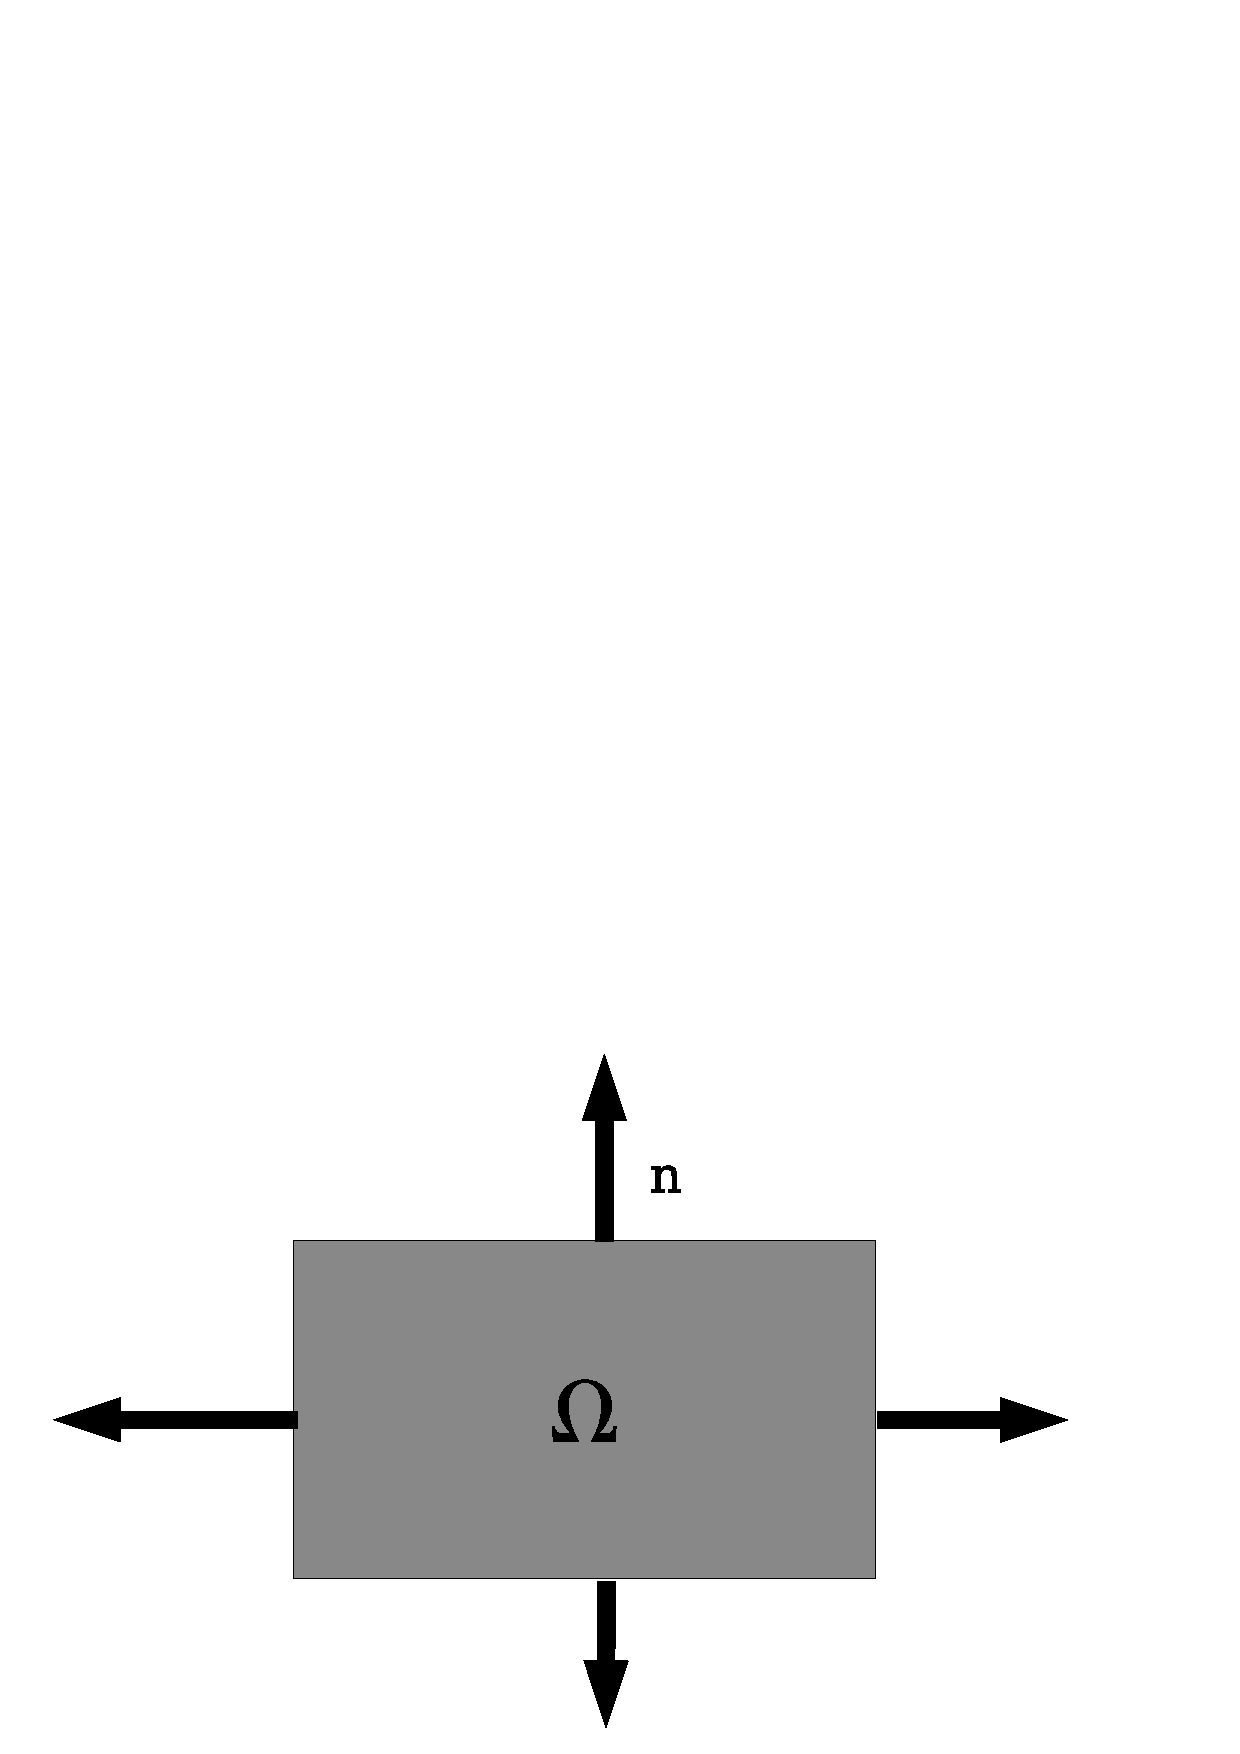
\includegraphics[width=\figwidth]{FirstStepDomain}}
\caption{Domain $\Omega$ with outer normal field $n$.}
\label{fig:FirstSteps.1}
\end{figure}

\begin{figure}
\centerline{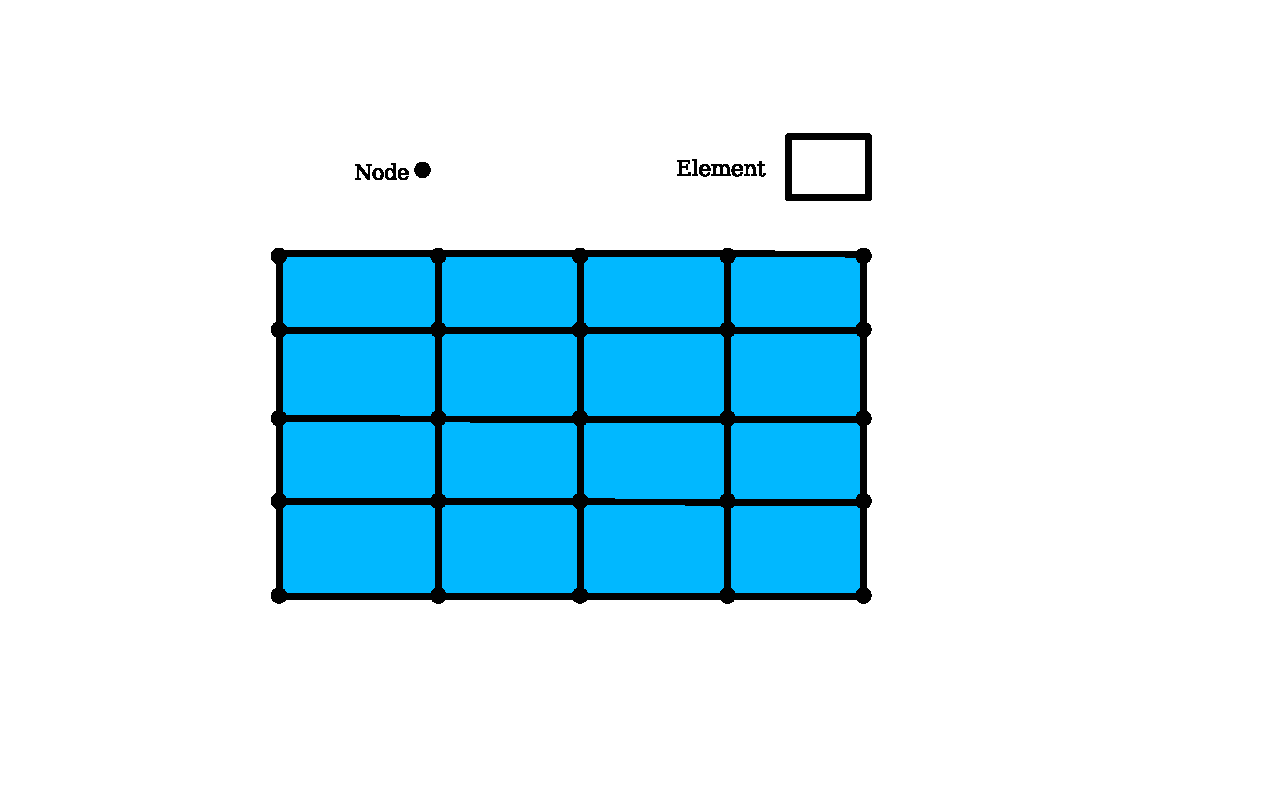
\includegraphics[width=\figwidth]{FirstStepMesh}}
\caption{Mesh of $4 \time 4$ elements on a rectangular domain.  Here
each element is a quadrilateral and described by four nodes, namely
the corner points. The solution is interpolated by a bi-linear
polynomial.}
\label{fig:FirstSteps.2}
\end{figure}

We want to solve the \index{partial differential equation}(\index{PDE})
\begin{equation}
-\Delta u + \alpha u =f 
\label{eq:FirstSteps.1}
\end{equation}
for the solution $u$ on the domain $\Omega$.  Here we assume that the
domain is the rectangle of length $1$ and height $2$, see
\fig{fig:FirstSteps.1}.  $\Delta$ denotes the \index{Laplace
operator} which is defined by
\begin{equation}
\Delta u = (u\hackscore {,1})\hackscore{,1}+(u\hackscore{,2})\hackscore{,2}
\label{eq:FirstSteps.1.1}
\end{equation}
where for any function $w$ and any direction $i$ $u\hackscore{,i}$
denotes the derivative of $w$ with respect to $i$.  $\alpha$ is a
known constant (we will set $\alpha=10$) and $f$ is a given function
which may depend on the location in the domain.  On the boundary of
the domain $\Omega$ the solution $u$ shall fulfill the so-called
homogeneous \index{Neumann boundary condition}
\begin{equation}
\frac{\partial u}{\partial n} = 0
\label{eq:FirstSteps.2}
\end{equation}
where $n=(n\hackscore1,n\hackscore2)$ denotes the outer normal field
of the domain, see Figure~\ref{fig:FirstSteps.1} and
\begin{equation}
\frac{\partial u}{\partial n} = n\hackscore1 u\hackscore{,1} +
n\hackscore2 u\hackscore{,2}
\label{eq:FirstSteps.2.1}
\end{equation}
denotes the normal derivative on the boundary.  The partial
differential \eqn{eq:FirstSteps.1}) together with the
boundary condition~(\eqn{eq:FirstSteps.2}) forms a boundary value
problem (\index{BVP}) for unknown function $u$.

In most cases, the BVP cannot be solved analytically and numerical
methods have to be used construct an approximation of the solution
$u$. Here we will use the \index{finite element method}
(\index{FEM}). The basic idea is to fill the domain with a set of
points, so called nodes. The solution is approximated by its values on
the nodes. Moreover, the domain is subdivide into small subdomain,
so-called elements. On each element the solution is represented by a
polynomial of a certain degree through its values at the nodes located
in the element. The nodes and its connection through elements is
called a \index{mesh}.  \fig{fig:FirstSteps.2} shows an example
of a FEM mesh with four elements in the $x_0$ and for elements in the
$x_1$ direction over a rectangular domain. On more details we referring
to the literature, for instance \cite{X1,X2,X3}.

\escript provides the class \linearPDE to define a
general linear, steady differential partial differential equation of
second order. We will discuss the most general form that can be
defined through \class{linearPDE} later. The components which are
relevant for us here is as follows:
\begin{equation}
-\sum\hackscore{i,j=0}^k (A\hackscore{ij}
 u\hackscore{,j})\hackscore{,i} + D u = Y
\label{eq:FirstSteps.3}
\end{equation}
In this form $D$ and $Y$ are scalars and $A$ is a $k \times k$ matrix
where $k$ denotes the spatial dimension (in our example we have
$k=2$).  By comparing the template~(\ref{eq:FirstSteps.3}) with the
differential equation~(\ref{eq:FirstSteps.1}) we want to solve we can
immediately identify the appropriate values for $A$, $D$ and $Y$:
\begin{equation}
\begin{array}{lcccc}
A\hackscore{ij} & = & \delta\hackscore{ij}&  =&
                 \left[
                                  \begin{array}{cc}
                                  1 & 0\\
                                  0 & 1
                                  \end{array}
                 \right] \\
D & =& \alpha \\
Y & = & f \\
\end{array}
\label{eq:FirstSteps.3.1}
\end{equation}
When the PDE is defined via~(\eqn{eq:FirstSteps.3}), \class{linearPDE}
makes a particular assumptions about the boundary conditions:
\begin{equation}
-\sum\hackscore{i,j=0}^k n\hackscore{i} A\hackscore{ij}
 u\hackscore{,j} = 0
\label{eq:FirstSteps.4}
\end{equation}
Note that this boundary condition does not require extra information
as it only refers to the coefficient $A$ which already appears in the
PDE and so natural for it. Therefore this boundary condition is called
a \index{natural boundary condition}.

We will set $\alpha=10$ and $f=10$ such that $u=1$ becomes the exact
solution of the boundary value problem.  We make this very simple
choice to be able to test our program as we can compare the result
with the exact solution. Later we will set $\alpha$ and $f$ to
functions of their locations in the domain in which case we will not
be able to give an analytic solution. However, after testing our
program on this very simple case, we can be confident that it working
correctly before we apply it is a more complicated situation.

This is the program to solve the boundary value problem: (Remember that
lines starting with '\#' are commend lines in Python)
%\verbatiminput{examples/FirstSteps1.py}
\begin{python}
# import ESyS and finley
from ESyS import *
import finley
# set a value for alpha:
alpha=10
# generate mesh:
mydomain=finley.Rectangle(n0=40,n1=20,l0=2.,l1=1.)
# generate a system:
mypde=linearPDE(A=[[1,0],[0,1]],D=alpha,Y=10,domain=mydomain)
# generate a test solution:
u=mypde.getSolution()
# calculate the error of the solution
error=u-1.
print "norm of the approximation error is ",Lsup(error)
\end{python}
Line 2 import \escript and a few other tools for \ESyS. In Line 3 is
importing \finley which is used to solve the partial differential
equation. In line 7, a rectangular domain of length $l\hackscore 0=2$
and height $l\hackscore 1=1$ is generated and subdivided in
$n\hackscore 0=40$ and $n\hackscore 1=20$ elements in $x\hackscore 0$
and $x\hackscore 1$ direction, respectively.

We are using a function of \finley. This determines later in the code
which solver for the PDE is actually being used to solve the PDE.

The solution is done in three steps:
\begin{enumerate}
\item generate a finite element mesh subdividing the domain into elements.
\item assemble the system of linear equations $Mu=b$ from the BVP
\item solve the linear system to get $u$
\end{enumerate}
The returned $u$ is given an approximation of the solution of the BVP
at the nodes of the finite element mesh. The quality of the
approximation depends on the size of the elements of the finite
element mesh: As smaller the element size the better the
approximation.  In our example we know the solution of the BVP so we
can compare the returned approximation with the true solution.  In
fact, as the true solution is simple, we can expect that the
approximation is exact.

The first step imports the package \ESyS which includes among
others the module \finley.

\section{A Time Dependent Problem}

% \verbatiminput{exam/finley\hackscoretime.py}

\section{With Dirichlet Conditions}

% \verbatiminput{exam/finley\hackscoredirichlet.py}

\section{Systems of PDEs}

% \verbatiminput{exam/system\hackscoretime.py}

\section{Explicit Schemes}
% \verbatiminput{exam/explicit\hackscoretime.py}
